\chapter{Thermodynamic favorability of thermophile lipid chain modifications across a temperature and redox gradient}\label{ch2}

\section{Introduction}


Ongoing efforts are needed to elucidate the factors that ultimately control lipid distribution in the environment. We have a general understanding of how certain lipid adaptations are supposed to work (e.g. chain length and cis double bonds in regulating membrane fluidity and permeability, ether bonds in resisting acid hydrolysis, etc.), though we are still discovering how various lipid structural characteristics function (e.g. isoprenoidal methylation, GDGT rings) and the function of some structures are almost completely unknown (BHP side chains). Lipids obviously need to function for an organism, but it must also have an acceptable biosynthetic cost. Each lipid structure has an energetic cost associated with its synthesis and modification, which may potentially change across an environmental gradient based on temperature and the chemical or redox composition of the surroundings. Evolution will tend to select for lipid structures that confer fitness advantage according to this cost/benefit analysis. Example studies (for lipids functioning while having an acceptable cost): substituting nitrogen for phosphorus, etc. 




While it has been repeatedly shown that certain lipid modifications or adaptations regulate cellular membrane fluidity and thermostability, little attention has been paid to the energetic consequences of adopting one strategy versus another within the thermal and geochemical context of an organism's surroundings. After all, biology is composed of chemical systems, and differences in the habitat thermochemistry will affect which metabolic and biosynthetic pathways are more or less favorable.  Fundamental examples include the conversion of nutrients (for chemotrophs) or photons (for phototrophs) into cellular energy. If a food source or sunlight is taken away, the generation of energy using those particular biochemical pathways becomes unfavorable. This is a central theme of countless experiments involving microbial cultures in various growth conditions, though fewer studies have addressed the potential energetic favorability of synthesizing one biomolecular structure, such as a lipid with a particular headgroup or chain modification, relative to other homologous functional structures.

Some organisms have adapted strategies to synthesize homologous `alternate' versions of biomolecules in response to nutrient limitation. It was shown, for instance, that xxx begins synthesizing lipids with amino acid headgroups when phosphorus concentrations are limiting enough for phospholipid biosynthesis to become unfavorable (ref) and that alternate nitrogenases may be synthesized by some nitrogen-fixing bacteria to utilize alternate metal cofactors in environments where the `preferred' metal is scarce. It makes intuitive sense that nutrient limitation can lead to an insufficient supply of the raw biosynthetic materials needed for normal cell function, and that adopting alternate biomolecules is one strategy to deal with the problem. It also makes sense that prolonged exposure to environmental stresses drives the evolution of existing metabolic and biosynthetic pathways, leading to the diversity of physiological and biochemical strategies that organisms employ in nature.

Despite the intuitive logic that an organism's biochemistry and habitat are intimately linked, it has proven difficult to quantitatively define relative favorability of metabolic and biosynethetic pathways across different environmental thermochemical compositions. The reasons for this stem from our incomplete knowledge regarding (and inability to accurately measure) the details of energy supply and demand at the cellular level.

Take two microorganisms which have considerably different bioenergetic strategies - a hyperthermophilic bacterium of the genus \textit{Thermocrinis} and a thermophilic cyanobacterium of the genus \textit{Synechococcus}. The former lives between (xxx temperature range) and relies exclusively on chemical energy supplied to it by its environment, while the latter lives (xxx temperature range) and utilizes sunlight. Both organisms are suited to the particular set of environmental conditions of their habitat, having evolved different suites of biomolecules necessary for growth and division. The sunlight-harvesting thylakoid membranes of \textit{Synechococcus} become leaky and unstable when exposed to the extreme temperatures where \textit{Thermocrinis} thrives (refs), whereas the abundant energy afforded by oxygenic photosynthesis conceivably allows \textit{Synechococcus} to outcompete \textit{Thermocrinis} at lower temperatures.  Transitions from  \textit{Themocrinis}-dominated to  \textit{Synechococcus}-dominated microbial communities exist in nature and can be visually abrupt in streams that trickle from silica-rich alkaline hot springs such as Bison Pool, Mound Spring, and Octopus Spring in Yellowstone National Park (YNP), USA. 

An enormous proportion of cellular energy is spent by microorganisms to accumulate nutrients and energy for growth and division. For primary producers such as \textit{Thermocrinis} and \textit{Synechococcus}, this involves regular synthesis of every biomolecule in a new cell from bioavailable chemical species such as inorganic carbon, ammonia or N\textsubscript{2}, sulfide, phosphate, and additional trace nutrients supplied by the surroundings. Every energetic shortcut and nutrient-saving biomolecular structure that eventually results in a competitive new cell is conceivably favored through evolutionary selection. The form taken by these cost-saving metabolic shortcuts and structures depends on the thermal and chemical conditions of the habitat. An energy-saving strategy employed in one set of environmental conditions may be less viable in another. If \textit{Synechococcus} is moved above its maximum temperature threshold, its biomolecular assemblage can no longer maintain stability and the cell dies and falls apart. If \textit{Thermocrinis} is moved to a lower temperature, its biomolecular configuation may conceivably allow it to maintain a stable (living) state, though in the long run it would be outcompeted by the assemblage of biomolecules forming a \textit{Synechococcus}-dominated community, which are in a more stable configuration within that lower temperature regime. In other words, the range of environmental conditions that permit a living, energetically favorable state depends upon the chemical composition and configuration of a cell's biomolecular assemblage, which in turn is a result of evolutionary adaptation.

With this perspective, it is possible to approach the original problem of quantifying `bioenergetic favorability' by examining bulk, community-level assemblages of microbial biomolecules found across environmental conditions and searching for trends in physiochemical properties that contribute to relative thermodynamic stability. One such trend that has been previously explored is the relative stabilities of homologous proteins along the thermal and geochemical gradient of Bison Pool, a terrestrial hot spring in Yellowstone National Park (Jeff's work)... where protein assemblages found to be most stable were the ones belonging to the microbial communities living in the environmental conditions most conducive to their biosynthesis from available inorganic chemical species. In other words, the most energetically favorable assemblage of homologous proteins predicted by thermodynamic calculations was usually very close to the assemblage observed in Bison Pool samples. One property found to correlate well with relative protein favorability was Z\textsubscript{C}, or the oxidation state of carbon averaged across the entire molecule of interest, with lower numbers indicating more reduced carbon (e.g. Z\textsubscript{C} of -4 in methane) and higher numbers indicating more oxidized carbon (e.g. Z\textsubscript{C} of +4 in carbon dioxide). For homologous proteins, Z\textsubscript{C} was found to be at its lowest (most reduced carbon) in the microbial community sampled at the source of Bison Pool, where hot, reduced fluids bubble up from the ground and trickle away along an outflow channel. Protein Z\textsubscript{C} progressively increases (becomes more oxidized) along downstream samples, coinciding with cooler, more oxidized fluids. Follow-up studies demonstrated that, among these homologous proteins, those with more reduced carbon (lower Z\textsubscript{C}) were indeed more energetically favorable in the hotter, reducing conditions close to the source than proteins with more oxidized carbon (higher Z\textsubscript{C}), which were instead favored in the cooler, more oxidizing fluids downstream.

The usefulness of Z\textsubscript{C} in predicting the relative energetic favorability of homologous biomolecules is enhanced by its relative ease of calculation, which requires little more than a chemical formula, or in the case of weighted Z\textsubscript{C}, additional knowledge of relative abundances of a biomolecule within a sample. The aforementioned studies on proteins relied on the copy number of peptides encoded in the metagenomes of microbial communities, and not on any measure of protein expression or abundance, so a weighted Z\textsubscript{C} could not be determined for proteins along Bison Pool.



\subsection{Sample-averaged free alkyl chains}
Various abundance-weighted structural characteristics of alkyl chains such as nC (number of aliphatic carbons), nUnsat (number of unsaturations), nOH (number of secondary hydroxylations), mole fraction of monolayer-forming chains and backbone-chain linkage types (ether, ester, amide, and C-C) were calculated from observed abundances of IPLs with Equation \ref{eq:avechain} in Chapter \ref{ch1} and are reported in Table \ref{tab:mods}. In this study, partial molal thermodynamic aqueous properties of eighteen hypothetical `site-averaged' alkyl chains were estimated, each representing the abundance-weighted structural characteristics of alkyl chains in a hot spring sample. For instance, the nC and nUnsat in sample BP1 was observed to be 19.80 and 3.12$\cdot$10\textsuperscript{-1}, respectively, so the thermodynamic properties estimated for the site-averaged alkyl chain representing BP1 assume a hypothetical chemical structure with 19.80 aliphatic carbons and 3.12$\cdot$10\textsuperscript{-1} unsaturations, and so on. This is equivalent to calculating thermodynamic properties for thousands of individual chains and then taking an abundance-weighted average of each property. It would not have been possible in this study to estimate the thermodynamic properties of every observed chain due to an inability to resolve structural characteristics of individual IPL alkyl chains using this LC-MS method. The rational for calculating thermodynamic properties from abundance-weighted structural characteristics was as follows: if an IPL observed in a sample has 38 aliphatic carbons and two unsaturations distributed between two chains, the structural characteristics of its chains must be described using averages without resorting to assumptions about which chain bears which combination of characteristics, and by extension, the estimated thermodynamic properties of alkyl chains must therefore be described by averages as well. This was taken a step further by assuming that the structural characteristics of all alkyl chains in a sample could be averaged for the sake of calculating thermodynamic properties, resulting the concept of a `sample-averaged' alkyl chain.

Other rationales: thermo properties of long-chain hydrocarbons change linearly with chain length, so why not have fractional chain length as a mathematical construct to describe an average alkyl chain in a sample? Similarly, the contribution of functional groups to the properties to these sorts of organic molecules is often additive, which serves as the foundation for group additivity theory for predicting thermodynamic properties. If one or two unsaturations can be added, and each unsaturation changes the estimated properties by the same amount each time, why not have a fractional unsaturation?

Other considerations: predicted thermodynamic properties are for `free' chains, as opposed to IPL-linked chains (point to figure). Free chains were used due to a lack of good amide bond data for organics other than amino acids, and also to pave the way for future work: future work could be to try this with esters, ethers, amide-bonded, C-C chains to see if results differ, and to see where the free chains are more/less stable than the linked chains (ethers in acid, anyone?).

Move this stuff to the intro.

% Previous Notes:

% Consider two sets of chemical assemblages representing all of the biomolecules that comprise a \textit{Thermocrinis} and \textit{Synechococcus} cell. Each assemblage has a cost associated with biosynthesis that depends on energy and nutrient availability.

% The example hypothesis given above for why \textit{Thermocrinis}-dominated bacterial communities transition to \textit{Synechococcus}-dominated as temperature drops is notably qualitative, and raises even more questions that depend on equally and unsatisfyingly qualitative answers.

% [] what is the energy gain difference between synthesizing one \textit{Synechococcus} cell compared to one \textit{Thermocrinis} cell from scratch (i.e. from bioavailable chemical species such as carbon dioxide, ammonia, sulfide, phosphate, and other nutrients dissolved in the flowing stream) at 70$\degree$C?


% [] can be set aside for one round of cell division in photosynethetic \textit{Synechococcus} compared to chemosynthetic \textit{Thermocrinis}, both at 70$\degree$C where photosynthesis can be carried out by \textit{Synechococcus}, assuming the new cells are synthesized completely from scratch; i.e. bioavailable dissolved chemical species such as CO2, ammonia, sulfide, phosphate, and other nutrients dissolved in the stream as it flows past? According to the aforementioned hypothesis, \textit{Synechococcus}'s ability to photosynthesize should allow it to accumulate more energy during the cell cycle and thereby allow it to outcompete \textit{Thermocrinis}, but even attempting to address this hypothesis experimentally to arrive at quantitative answers based on energy supply and demand.

% [] would require an enormous undertaking to simultaneously measure and compare the energy supplied by, and the cost of maintaining and duplicating, the biochemical framework of a \textit{Synechococcus} cell versus that of a \textit{Thermocrinis} cell, which is further complicated by the dynamic fluxes and cycles of energy and materials passed through the biogeochemical network of a natural system. Even if armed with accurate knowledge of the ATP or NAD(P)H yield/cost of any biosynthetic pathway, comparing the relatively 'energetic favorability' of synthesizing and maintaining a \textit{Synechococcus} cell versus a \textit{Thermocrinis} cell still depends entirely on the type, concentration, bioavailability, and efficiency in utilizing the nutrients and energy sources supplied by an environment at some temperature, pressure, and chemical composition.


%[The primary goal of geobiochemistry is to understand the influence of geology on biochemistry.
% - Redox gradients in nature. Changing chemical composition affects the energetic properties of chemical reactions. Because biology is composed of chemical systems, changing the chemistry of the environment means changing which reactions are more or less favorable - metabolic and biosynthetic pathways. It is well-known that organisms adapt their metabolism to obtain energy from their environment (dead otherwise). Fewer studies have focused on how the thermochemical conditions of a microbial habitat affects the energetic cost of synthesizing a particular biomolecule.]

\section{Methods}
\subsection{Analysis of water chemistry}
Sampling locations were metered and water samples were collected, filtered, and analyzed as described in Chapter \ref{ch1}. Briefly, temperature and pH were metered in the field as close to the sampling locations as possible using a YSI 30 conductivity meter for temperature and a model 3300i or 3110 WTW pH meter with WTW probe for pH. Concentrations of dissolved oxygen and sulfide were measured in unfiltered water samples using Hach 2400 or 2800 portable spectrophotometer with Hach reagents. Water samples collected for laboratory analyses were filtered with Supor (Pall Corporation) filters down to 0.2 microns; samples for ion chromatography were collected in 30 mL HDPE Nalgene bottles (two per sample) and stored at -20$^{\circ}$C before analysis on Dionex DX-600 systems for concentrations of major cations and anions.

Filtered samples for dissolved inorganic carbon (DIC) analysis were collected in acid-washed amber glass vials with black butyl rubber septa. DIC was chemically converted to CO\textsubscript{2} by reacting with phosphoric acid before analysis on an OI Wet Oxidation TOC analyzer coupled to a Thermo Delta Plus Advantage mass spectrometer as described in \cite{havig2011merging}.

\subsection{Analysis of environmental IPLs} Methods used to collect, identify, and quantify the hot spring microbial IPLs from sediments and biofilms are described in detail in Chapter \ref{ch1}. Briefly, sediments and biofilms were collected into sterile specimen containers with sterilized forceps and spatulas and stored on dry ice the field, and at -80$^{\circ}$C in the lab. Samples were freeze-dried, homogenized with mortar and pestle, and extracted for lipids using a modified version of the Bligh and Dyer method \citep{white1998signature}. Aliquots of the resulting total lipid extracts (TLEs) were analyzed using the hydrophilic interaction chromatography (HILIC) method \citep{Wrmer_Application_2013} on an Agilent 1200 series high performance liquid chromatograph (HPLC) attached to a Agilent 6520 Accurate-Mass Quadrupole Time-of-Flight Mass Spectrometer with an electrospray ionization source and operated in positive ion mode. Commercially-available standards were used to obtain response factors for calculating IPL mole fractions from mass spectral peak areas. Response factors are given in Table \ref{tab:RF} and response factor assignments to observed IPLs are reported in Table \ref{tab:IPL}.

\subsection{Deriving properties and chemical formulae of sample-averaged free alkyl chains}



Calculation of the elemental abundance of sample-averaged free alkyl chains began with the chemical formulae of sample-averaged IPL-linked alkyl chains, to which additional carbon, hydrogen, oxygen, and nitrogen were added to convert ether-linked chains into free fatty alcohols, ester-linked chains into free fatty acids, amide-linked chains into free fatty amides, and CC-linked chains into free methyl-capped chains. Chemical formulae of sample-averaged IPL-linked alkyl chains and mole fractions of alkyl chain linkage types required for these calculations are reported in Table \ref{tab:leftover_props} for isoprenoidal chains and \cite{boyer2018thermophile} for all others. Chemical formulae of sample-averaged free alkyl chains are reported in Table \ref{tab:IPL_thermo}.

The number of carbon atoms ($c_{free}$) in the chemical formulae of sample-averaged free alkyl chains was calculated with

\begin{equation}
    c_{free} = c_{linked} + x_{cc}
\end{equation}

\noindent where $c_{linked}$ indicates the number of carbon atoms in the sample-averaged IPL-linked alkyl chain of the sample, and $x_{cc}$ stands for the observed mole fraction of CC-linked alkyl chains. Addition of a number of carbons equal to $x_{cc}$ to $c_{linked}$ accounts for the carbon that would be gained with a terminal methyl group assuming hypothetical carbon-carbon bond breakage of CC-linked alkyl chains to produce the sample-averaged free chains considered in this study.

The number of hydrogen atoms ($h_{free}$) in the chemical formulae of sample-averaged free alkyl chains was calculated with

\begin{align}
\begin{split}
    h_{free} = &h_{linked} + x_{ether} + x_{ester}\\
        & + 2(x_{amide}) + 3(x_{cc}) \\
\end{split}
\end{align}

\noindent where $h_{linked}$ represents the number of hydrogen atoms in the sample-averaged IPL-linked alkyl chain of the sample, and $x_{ether}$, $x_{ester}$, and $x_{amide}$ correspond to the observed mole fractions of ether-, ester-, and amide-linked alkyl chains, respectively. A number of hydrogens equal to $x_{ether}$ and $x_{ester}$ are added to $h_{linked}$ to account for the single hydrogen in the hydroxyl groups of the resulting alcohol and carboxylic acid group assuming hypothetical hydrolysis of ether- and ester-linked chains to produce free fatty acids and fatty alcohols. Similarly, two times $x_{amide}$ is added to account for the two hydrogen atoms in the amine group of the free amide after the hypothetical hydrolysis of an amide-linked chain. Lastly, adding a number of hydrogens equal to three times $x_{cc}$ accounts for the three hydrogen atoms added by a terminal methyl group after the hypothetical carbon-carbon breakage of a CC-linked alkyl chain.

The number of nitrogen atoms ($n_{free}$) in the chemical formulae of sample-averaged free alkyl chains was calculated with

\begin{equation}
    n_{free} = n_{linked} + x_{amide}
\end{equation}

\noindent where $n_{linked}$ indicates the number of nitrogen atoms in the sample-averaged IPL-linked alkyl chain. A number of nitrogen atoms equal to $x_{amide}$ is added to $n_{linked}$ to account for the single nitrogen atom added by the amine group of the free amide after hypothetical hydrolysis of an amide-linked alkyl chain.

The number of oxygen atoms ($o_{free}$) in the chemical formulae of sample-averaged free alkyl chains was calculated with

\begin{equation}
    o_{free} = o_{linked} + x_{ether} + x_{ester}
\end{equation}

\noindent where $o_{linked}$ is the number of oxygen atoms in the sample-averaged IPL-linked alkyl chain. A number of oxygen atoms equal to $x_{ether}$ and $x_{ester}$ are added to $o_{linked}$ to account for the single oxygen atom in the hydroxyl groups of the resulting alcohol and carboxylic acid group assuming hypothetical hydrolysis of ether- and ester-linked chains to produce free fatty acids and fatty alcohols.

\subsection{Calculation of thermodynamic properties}
Partial molal thermodynamic properties $\Delta_{f}G_{aq}^{\circ}$, $\Delta_{f}H_{aq}^{\circ}$, $V_{aq}^{\circ}$, $Cp_{aq}^{\circ}$, $\Delta_{h}G^{\circ}$, of sample-averaged free alkyl chains were estimated using the equation

\begin{align}
\begin{split}
\Xi_{chain} = & (m_{alcohol}\cdot \text{nC} + b_{alcohol})(x_{ether}) \\
            + & (m_{acid}\cdot \text{nC} + b_{acid})(x_{ester}) \\
            + & (m_{alkane}\cdot \text{nC} + b_{alkane})(x_{cc}) \\
            + & (m_{acid}\cdot \text{nC} + b_{acid})(x_{amide}) \\
            + & (\Delta\Xi_{amide})(x_{amide}) \\
            + & (\Delta\Xi_{unsat})(\text{nUnsat}) \\
            + & (\Delta\Xi_{hydroxyl})(\text{nOH}) \\
            + & (\Delta\Xi_{pent})(\text{nPent}) \\
            + & (\Delta\Xi_{hex})(\text{nHex}) \\
            + & (\Delta\Xi_{monolayer})(x_{GDGT}) \\
            + & (\Delta\Xi_{methyl})(\text{nMethyl}) \\
\end{split}
\end{align}



\noindent where $\Xi_{chain}$ designates the thermodynamic property to be estimated, $m_{alcohol}$, $m_{acid}$, $m_{alkane}$, $b_{alcohol}$, $b_{acid}$, $b_{alkane}$ correspond to the slopes ($m$) and intercepts ($b$) of linear regressions of the value of each thermodynamic property as a function of chain length for fatty acids, fatty alcohols, and alkanes given in Table \ref{tab:regress_chain_prop}, $x_{ether}$, $x_{ester}$, $x_{cc}$, and $x_{amide}$ represent the mole fractions of ether-linked, ester-linked, CC-linked, amide-linked, and GDGT alkyl chains observed in the sample, $x_{GDGT}$ corresponds to the mole fraction of alkyl chains belonging to GDGT given in Table \ref{tab:leftover_props},  nC, nUnsat, nHydrox, nPent, and nHex stand for the abundance-weighted average number of aliphatic carbons, unsaturations, hydroxylations, pentacyclic rings, and hexacyclic per alkyl chain observed in the sample, respectively, $\Delta\Xi_{amide}$ indicates the estimated difference in the thermodynamic property between a fatty amid and fatty acid taken from Table \ref{tab:amide}, $\Delta\Xi_{unsat}$ designates the estimated difference in the thermodynamic property between a monounsaturated and saturated chain taken from Table \ref{tab:unsat}, $\Delta\Xi_{hydroxyl}$ indicates the estimated difference in the thermodynamic property between a hydroxylated and nonhydroxylated chain taken from Table \ref{tab:grpadd_chain}, $\Delta\Xi_{pent}$ represents the estimated difference in the thermodynamic property between a chain with a pentacyclic ring and a noncyclic chain taken from Table \ref{tab:ring}, $\Delta\Xi_{hex}$ stands for the estimated difference in the thermodynamic property between a chain with a hexacyclic ring and a noncyclic chain taken from Table \ref{tab:ring}, $\Delta\Xi_{monolayer}$ corresponds to the estimated difference in the thermodynamic property between a monolayer-forming and bilayer-forming chain taken from Table \ref{tab:grpadd_chain}, $\Delta\Xi_{methyl}$ designates the estimated difference in the thermodynamic property between a methyl-branched and straight chain taken from Table \ref{tab:grpadd_chain}, and nMethyl represents the abundance-weighted number of methyl branches per alkyl chain. In this study, methyl branching could not be observed directly or quantified, therefore the value from nMethyl accounts only for methyl branching assumed present in isoprenoidally-derived alkyl chains, and as such should be interpreted as a minimum because non-isoprenoidal chains may also have methyl branching. The contribution of $\Delta\Xi_{methyl}$ tends to be minor relative to those from other alkyl chain modifications, so we do not expect variation due to uncertainty in nMethyl to have a considerable effect on $\Xi_{chain}$. The term nMethyl was estimated from

\begin{equation}
\text{nMethyl} = (\text{nC}/5 - \text{nPent} - \text{nHex})(x_{GDGT} + x_{AR})
\end{equation}

\noindent where $x_{AR}$ stands for the mole fraction of alkyl chains belonging to archaeol (AR), found in Table \ref{tab:leftover_props}. The term nC$/5$ is meant to account for one methyl branch per five carbons in isoprenoidally-derived alkyl chains, represented here as the sum of the mole fractions $x_{GDGT}$ and $x_{AR}$. Because each pentacyclic and hexacyclic ring incorporated into the alkyl chains of GDGTs replaces a methyl group, nPent and nHex are subtracted when determining number of methylations.


\subsection{Calculation of sample-averaged free alkyl chain percent speciation at hot spring conditions.} The revised Helgeson-Kirkham-Flowers (HKF) equation of state \citep{shock1992calculation} was used to predict equilibrium constants for reactions at the temperatures measured for the hot spring sample locations. Equation of state parameters, a\textsubscript{1}, a\textsubscript{2}, a\textsubscript{3}, a\textsubscript{4}, c\textsubscript{1}, c\textsubscript{2}, and $\omega$, for sample-averaged free alkyl chain are reported in Table \ref{tab:IPL_thermo} and were estimated according to the correlation strategies described in \cite{plyasunov2001correlation} for aqueous polar organic nonelectrolytes.

Predictions of aqueous free alkyl chain relative abundances assumes thermodynamic equilibrium between the chain and a set of basis species representing naturally available inorganic molecules relevant to autotrophic metabolism. The set of basis species used in this study consisted of bicarbonate (HCO\textsubscript{3}\textsuperscript{-}), ammonium (NH\textsubscript{4}\textsuperscript{+}), protons (H\textsuperscript{+}), electrons (e\textsuperscript{-}) and water (H\textsubscript{2}O). The only exception was made for calculations performed at the conditions of sample MS5; ammonium was below detection limit and was replaced by nitrate (NO\textsubscript{3}\textsuperscript{-}) as the nitrogen-bearing basis species.

Formation reactions from basis species were written for each aqueous free alkyl chain with a number of HCO\textsubscript{3}\textsuperscript{-}, NH\textsubscript{3}\textsuperscript{+}, H\textsuperscript{+} and e\textsuperscript{-} as reactants and water as a product, such that

\begin{equation}
    aHCO_{3}^{-} + bNH_{4}^{+} + cH^{+} + de^{-} = alkyl + fH_{2}O
\end{equation}

\noindent where $alkyl$ represents the elemental formula of the sample-averaged free alkyl chain (given in Table \ref{tab:IPL_thermo}), and $a$, $b$, $c$, $d$, and $f$ are stoichiometric reaction coefficients of the basis species required to balance the reaction.

sample-averaged free alkyl chains belonging to the same hot spring outflow channel (Bison Pool, Mound Spring, Empress Pool, and Octopus Spring) were grouped together for percent speciation calculations. Assuming metastable equilibrium, the activity of the $i^{th}$ alkyl chain of an outflow channel, $[alkyl_{i}]$ was estimated using the relation

\begin{equation} \label{eq:alkyl_activity}
\begin{split}
[alkyl_{i}] & = e^{A^{*}/RT}
\end{split}
\end{equation}

\noindent where $R$ is the gas constant, $T$ is temperature, and $A^{*}$ is `starred' reaction affinity defined as

\begin{equation}
A^{*} \equiv RT\ln{K/Q^{*}}
\end{equation}

\noindent where $K$ is the HKF-calculated equilibrium constant for the reaction and $Q^{*}$ is the `starred' reaction quotient comprised only of the activities of basis species. For the formation of sample-averaged alkyl chains,

\begin{equation}
Q^{*} = \frac{[H_{2}O]^{f}}{[HCO_{3}^{-}]^{a}[NH_{4}^{+}]^{b}[H^{+}]^{c}[e^{-}]^{d}}
\end{equation}

\noindent for all samples except for MS5, where $NH_{4}^{+}$ is replaced by $NO_{3}^{-}$. Activities of $NH_{4}^{+}$ and $NO_{3}^{-}$ were assumed to be equivalent to the molal concentrations of ammonia and nitrate reported in \cite{boyer2018thermophile}. Activities of protons were calculated directly from field pH measurements, while those of $HCO_{3}^{-}$ were calculated from DIC.

Metastable equilibrium percent abundance, $alkyl_{i}\%$, was calculated for the $i^{th}$ sample-averaged alkyl chain relative to others within the same hot spring using the equation

\begin{equation} \label{eq:percent_alkyl}
\begin{split}
alkyl_{i}\% & = \frac{[alkyl_{i}]}{\sum{[alkyl_{i}]}} \cdot 100\%.
\end{split}
\end{equation}

Thermodynamic analyses were performed in R with the package CHNOSZ \citep{dick2008calculation}. Calculations involving Equation \ref{eq:percent_alkyl} included the mosaic() function \citep{dick2017equilibrium}, allowing temperature- and pH-dependent speciation of basis species such that bicarbonate could fully or partially speciate into carbon dioxide or carbonate, and ammonium into ammonia, when calculating $K$ and $Q^{*}$. In the case of sample MS5 where nitrate was used in place of ammonia, nitrate was not allowed to speciate.

The concentration of electrons in $Q^{*}$ was used as the independent variable when solving for $alkyl_{i}\%$, allowing for metatable equilibrium percent abundances of sample-averaged free alkyl chains to change as a function of Eh. A resolution of 800 calculations across a range of Eh -0.56 to -0.30 volts for samples in Bison Pool and Octopus Spring, -0.70 to -0.40 volts for samples in Mound Spring, and -0.50 to -0.26 volts for samples in Empress Pool. These Eh ranges were selected to contain important changes in percent alkyl chain speciation across the temperatures and basis species concentrations of all samples within the outflow channel of a given hot spring.

Alkyl chain-predicted Eh was taken to be the Eh value, in volts, that results in a local maximum in percent abundance at the temperature and basis species concentrations of its own sample (e.g. the Eh that maximizes $alkyl_{BP2}\%$ at the temperature and $HCO_{3}^{-}$, $NH_{4}^{+}$, and $H^{+}$ concentrations measured at BP2). For samples without a local maximum in alkyl chain-predicted Eh, namely the first and last samples in a hot spring (e.g. BP1 and BP6 for Bison Pool), a percent abundance cutoff of 95\% was used instead.

A water sample could not be collected for ES2 during the 2012 field season. Because of this, concentrations of bicarbonate and ammonium are unknown and lipid-predicted Eh cannot be calculated for this sample.

\subsection{Sensitivity analysis} The sensitivity of thermodynamic predictions of sample-averaged free alkyl chain percent abundance to potential sources of analytical uncertainty was tested using the Monte Carlo-style partial randomization of underlying lipid data described in \cite{boyer2018thermophile}, where all LC-MS IPL peak areas were varied randomly up to a maximum of $\pm30\%$ and slopes of calibration curves up to a maximum of 0.01$\times$ and 100$\times$ and IPLs re-quantified over the course of 999 iterations. In this work, $alkyl_{i}\%$ was calculated for each sample-averaged free alkyl chain in each iteration as a function of Eh using a resolution of 400 calculations for the temperature and basis species concentrations of each sample.

\section{Results}
\paragraph*{Relative abundances of representative lipid chains} 


% example:
\begin{align}
\begin{split}
    19.8HCO_{3}^{-} + &0.0111NH_{4}^{+}\\
    + 135.9467H^{+} &+ 116.1467e^{-}\\
    &= alkyl_{BP1} + 58.14H_{2}O
\end{split}
\end{align}

\begin{itemize}

    \item Figure showing an average chain (e.g. online blue chemical cartoon). This is more like a figure that would appear in the introduction.
    
\end{itemize}


\section{Discussion}


% \section{Notes}
% When balance is set to 1 using equilibrate() in CHNOSZ, relative lipid activities are solved using a Boltzmann distribution. The following derives it from 

% \begin{equation*} \label{eq1}
% \begin{split}
% A & = RT\ln{(K/Q)} \\
% A/RT & = \ln{(K/Q)} \\
% & = \ln{K} - \ln{Q} \\
% & = \ln{K} - \ln{\frac{[a_{i}]^{1}[products]^{x}}{[reactants]^{y}}} \\
% & = \ln{K} - (\ln{\frac{[products]^{x}}{[reactants]^{y}}} + \ln{a_{i}}) \\
% & = \ln{K} - (\ln{Q^{*}} + \ln{a_{i}}) \\
% & = \ln{K} - \ln{Q^{*}} - \ln{a_{i}} \\
% & = A^{*}/RT - \ln{a_{i}}
% \end{split}
% \end{equation*}

% Assuming metastable equilibrium, $A$ = 0,
% \begin{equation*} \label{eq2}
% \begin{split}
% 0 & = A^{*}/RT - \ln{a_{i}} \\
% a_{i} & = e^{A^{*}/RT}
% \end{split}
% \end{equation*}

% Solving for degree of formation yields the Boltzmann distribution:
% \begin{equation*} \label{eq3}
% \begin{split}
% \frac{a_{i}}{\sum a_{i}} & = \frac{e^{A^{*}/RT}}{\sum{e^{A^{*}/RT}}}
% \end{split}
% \end{equation*}

% \begin{equation} \label{eq1}
% \begin{split}
% Q & = \frac{[a_{i}]^{1}[products]^{x}}{[reactants]^{y}} \\
% Q^{*} & = \frac{[products]^{x}}{[reactants]^{y}} \\
% A & = RT\ln{K/Q} \\
% A^{*} & = RT\ln{K/Q^{*}}
% \end{split}
% \end{equation}

%%%%



\singlespace
\begin{table}
\centering
\begin{adjustbox}{width=\textwidth,keepaspectratio}
\begin{threeparttable}
  \caption{Summary of abundance-weighted structural characteristics of isoprenoidal alkyl chains}




% Table generated by Excel2LaTeX from sheet 'leftover isoprenoidal props'
\begin{tabular}{clllcc}
\toprule
Site  & Sample & \multicolumn{1}{c}{$x_{AR}$} & \multicolumn{1}{c}{$x_{GDGT}$} & nPent & nHex \\
\midrule
Bison & BP1   & 1.98$\cdot 10$\textsuperscript{-2} & 4.90$\cdot 10$\textsuperscript{-1} & 2.24$\cdot 10$\textsuperscript{-1} &  \\
Pool  & BP2   & 2.30$\cdot 10$\textsuperscript{-2} & 3.00$\cdot 10$\textsuperscript{-1} & 1.63$\cdot 10$\textsuperscript{-1} &  \\
      & BP3   & 1.49$\cdot 10$\textsuperscript{-3} & 8.81$\cdot 10$\textsuperscript{-2} & 6.19$\cdot 10$\textsuperscript{-2} &  \\
      & BP4   &       & 7.16$\cdot 10$\textsuperscript{-3} & 5.52$\cdot 10$\textsuperscript{-3} &  \\
      & BP5   & 5.06$\cdot 10$\textsuperscript{-6} & 7.20$\cdot 10$\textsuperscript{-4} & 5.69$\cdot 10$\textsuperscript{-4} &  \\
      & BP6   &       & 2.94$\cdot 10$\textsuperscript{-3} & 2.40$\cdot 10$\textsuperscript{-3} &  \\
      &       &       &       &       &  \\
Mound & MS1   &       & 9.99$\cdot 10$\textsuperscript{-1} & 6.16$\cdot 10$\textsuperscript{-1} & 2.68$\cdot 10$\textsuperscript{-3} \\
Spring & MS2   & 2.30$\cdot 10$\textsuperscript{-2} & 6.07$\cdot 10$\textsuperscript{-1} & 3.01$\cdot 10$\textsuperscript{-1} &  \\
      & MS3   &       & 1.64$\cdot 10$\textsuperscript{-1} & 1.13$\cdot 10$\textsuperscript{-1} &  \\
      & MS4   &       & 5.85$\cdot 10$\textsuperscript{-2} & 4.25$\cdot 10$\textsuperscript{-2} &  \\
      & MS5   &       & 1.09$\cdot 10$\textsuperscript{-2} & 9.65$\cdot 10$\textsuperscript{-3} &  \\
      &       &       &       &       &  \\
Empress & EP1   & 1.97$\cdot 10$\textsuperscript{-2} & 8.63$\cdot 10$\textsuperscript{-1} & 4.45$\cdot 10$\textsuperscript{-1} & 1.09$\cdot 10$\textsuperscript{-2} \\
Pool  & EP2   & 4.74$\cdot 10$\textsuperscript{-3} & 4.71$\cdot 10$\textsuperscript{-1} & 2.91$\cdot 10$\textsuperscript{-1} & 7.83$\cdot 10$\textsuperscript{-3} \\
      & EP3   & 2.21$\cdot 10$\textsuperscript{-3} & 6.06$\cdot 10$\textsuperscript{-1} & 3.61$\cdot 10$\textsuperscript{-1} & 1.15$\cdot 10$\textsuperscript{-2} \\
      & EP4   & 4.08$\cdot 10$\textsuperscript{-3} & 2.31$\cdot 10$\textsuperscript{-1} & 1.43$\cdot 10$\textsuperscript{-1} & 2.98$\cdot 10$\textsuperscript{-3} \\
      & EP5   & 2.78$\cdot 10$\textsuperscript{-3} & 1.26$\cdot 10$\textsuperscript{-1} & 7.19$\cdot 10$\textsuperscript{-2} & 1.12$\cdot 10$\textsuperscript{-3} \\
      &       &       &       &       &  \\
Octopus & OS1   & 1.26$\cdot 10$\textsuperscript{-1} & 4.21$\cdot 10$\textsuperscript{-1} & 1.20$\cdot 10$\textsuperscript{-1} &  \\
Spring & OS2   & 5.08$\cdot 10$\textsuperscript{-6} & 7.60$\cdot 10$\textsuperscript{-3} & 4.21$\cdot 10$\textsuperscript{-3} & 1.46$\cdot 10$\textsuperscript{-4} \\
\bottomrule
\end{tabular}%




  
  \begin{tablenotes}
    % The order of footnotes here will determine their letter in the table
    

        
  \end{tablenotes}
  
  \label{tab:leftover_props}
  \end{threeparttable}
  \end{adjustbox}
\end{table}
\setcounter{tabcounter}{0} % reset custom table footnote counter
\doublespace





\singlespace
\begin{table}
\centering
\begin{adjustbox}{height=\textheight,keepaspectratio}
\begin{threeparttable}
  \caption{Partial molal thermodynamic aqueous and hydration properties of aliphatic carboxylic acids, alcohols, and alkanes with nC $>$ 2 used in the estimation of saturated fatty acid, fatty alcohol, and fatty hydrocarbon properties.}



% Table generated by Excel2LaTeX from sheet 'linkage thermo table'
\begin{tabular}{lrrrrr}
\toprule
      & $\Delta_{f}G^{\circ}_{aq}$\rtr{linkage_kjpermol} & $\Delta_{f}H^{\circ}_{aq}$\rtr{linkage_kjpermol} & $Cp^{\circ}_{aq}$\rtr{linkage_jpermolk} & $V^{\circ}_{aq}$\rtr{linkage_cm3permol} & $\Delta_{h}G^{\circ}$\rtr{linkage_kjpermol} \\
\midrule
propanoic acid & -390.99 & -512.41 & 253   & 67.9  & -21.4\rtr{khan1992henry} \\
n-butanoic acid & -381.62 & -535.34 & 337   & 84.61 & -20.9\rtr{khan1992henry} \\
n-pentanoic acid & -373.38 & -559.36 & 432.2 & 100.5 & -19.0\rtr{khan1992henry} \\
n-hexanoic acid & -364.51 & -582.79 & 523.0 & 116.55 & -17.8\rtr{khan1992henry} \\
n-heptanoic acid & -356.48 & -607.01 & 611.7 & 131.6 &  \\
n-octanoic acid & -349.15 & -631.99 & 700.4 & 147.4 &  \\
n-nonanoic acid & -339.82 & -654.92 & 789.1 & 163.2 &  \\
n-decanoic acid & -331.25 & -678.64 & 877.8 & 179.0 &  \\
n-undecanoic acid & -322.71 & -702.37 & 966.5 & 194.8 &  \\
n-dodecanoic acid & -314.13 & -726.09 & 1055  & 210.6 &  \\
1-propanol & -172.07 & -312.74 & 355   & 70.71 & -12.36 \\
1-butanol & -162.40 & -336.53 & 443   & 86.53 & -11.86 \\
1-pentanol & -151.72 & -359.56 & 535   & 102.50 & -11.11 \\
1-hexanol & -143.31 & -383.79 & 617   & 118.46 & -10.30 \\
1-heptanol & -134.41 & -408.39 & 702   & 133.03 & -9.72 \\
1-octanol & -123.93 & -429.85 & 778   & 151.20 & -9.14 \\
1-nonanol & -115.24 & -454.67 & 865   & 164.55 & -8.36 \\
1-decanol & -106.23 & -478.75 & 950   & 180.16 & -8.18 \\
1-undecanol & -96.52 & -502.77 & 1034  & 195.77 & -6.90 \\
1-dodecanol & -86.17 & -525.73 & 1119  & 211.38 & -6.04 \\
propane & -8.22 & -127.43 & 398   & 69.31 & 16.09 \\
n-butane & 0.24  & -151.53 & 482   & 75.55 & 16.58 \\
n-pentane & 8.88  & -175.45 & 573   & 99.07 & 17.52 \\
n-hexane & 19.26 & -198.69 & 636   & 114.68 & 18.26 \\
n-heptane & 27.45 & -224.54 & 739   & 130.29 & 18.95 \\
n-octane & 36.08 & -250.45 & 824   & 145.90 & 19.64 \\
n-nonane & 46.24 & -275.24 & 908   & 161.51 & 20.51 \\
n-decane & 55.50 & -296.34 & 993   & 177.12 & 21.24 \\
n-undecane & 64.71 & -321.12 & 1078  & 192.73 & 22.94 \\
n-dodecane & 74.65 & -343.26 & 1163  & 208.34 & 22.51 \\
n-tridecane & 81.58 & -368.84 & 1248  & 223.95 & 22.87 \\
n-tetradecane & 90.85 & -392.99 & 1333  & 239.56 & 23.55 \\
\bottomrule
\end{tabular}%


  
  \begin{tablenotes}
    % The order of footnotes here will determine their letter in the table
    Carboxylic acid properties are taken from \cite{shock1995organic} unless otherwise noted. Properties for alcohols and alkanes are recommended values from the ORganic Compounds HYDration properties (ORCHYD) database compiled by \cite{plyasunova2004database}.
    
    \tr{linkage_kjpermol} kJ mol\textsuperscript{-1},
    \tr{linkage_jpermolk} J mol\textsuperscript{-1} K\textsuperscript{-1},
    \tr{linkage_cm3permol} cm\textsuperscript{3} mol\textsuperscript{-1},
    \tr{khan1992henry} values calculated from Henry's law constants, $K_{H}$, reported in \cite{khan1992henry} using the relation $\Delta_{h}G^{\circ} = -RT\ln{K_{H}}$.
        
  \end{tablenotes}
  
  \label{tab:carbacid_alc_alk_props}
  \end{threeparttable}
  \end{adjustbox}
\end{table}
\setcounter{tabcounter}{0} % reset custom table footnote counter
\doublespace



\singlespace
\begin{table}
\centering
% \begin{adjustbox}{width=\textheight,keepaspectratio}
\begin{threeparttable}
  \caption{Partial molal thermodynamic aqueous and hydration properties of functional groups and chemical species used in the estimation of fatty amide properties.}



% Table generated by Excel2LaTeX from sheet 'fatty amide table'
\begin{tabular}{lrrrrr}
\toprule
      & $\Delta_{f}G^{\circ}_{aq}$\rtr{linkage_kjpermol} & $\Delta_{f}H^{\circ}_{aq}$\rtr{linkage_kjpermol} & $Cp^{\circ}_{aq}$\rtr{linkage_jpermolk} & $V^{\circ}_{aq}$\rtr{linkage_cm3permol} & $\Delta_{h}G^{\circ}$\rtr{linkage_kjpermol} \\
\midrule
$\lbrack$-CONH\textsubscript{2}$\rbrack$ & -194.8\rtr{amide_dick2006temperature} & -257.0\rtr{amide_dick2006temperature} & 21\rtr{amide_dick2006temperature} & 28.2\rtr{amide_dick2006temperature} &  \\
$\lbrack$-COOH$\rbrack$ & -387.3\rtr{amide_dick2006temperature} & -436.7\rtr{amide_dick2006temperature} & 22\rtr{amide_dick2006temperature} & 24.5\rtr{amide_dick2006temperature} &  \\
acetamide &       &       &       &       & -32.7\rtr{amide_sedlbauer2012database} \\
acetic acid &       &       &       &       & -21.0\rtr{amide_khan1992henry} \\
\midrule
$\Delta\Xi_{amide}$ & 192.5\rtr{amide_groupsubtract} & 179.7\rtr{amide_groupsubtract} & -1\rtr{amide_groupsubtract} & 3.7\rtr{amide_groupsubtract} & -11.7\rtr{amide_acetamidesubtract} \\
\bottomrule
\end{tabular}%



  
  \begin{tablenotes}
    % The order of footnotes here will determine their letter in the table

    \tr{amide_kjpermol} kJ mol\textsuperscript{-1},
    \tr{amide_jpermolk} J mol\textsuperscript{-1} K\textsuperscript{-1},
    \tr{amide_cm3permol} cm\textsuperscript{3} mol\textsuperscript{-1},
    \tr{amide_dick2006temperature} \cite{dick2006temperature},
    \tr{amide_sedlbauer2012database} value from \cite{cabani1981group} with an adjustment of +7.9 kJ/mol to convert the standard state definition used by the authors for gases (1M ideal gas) to those used here (pure ideal gas) when deriving properties of the hydration process, as reported in the \textit{Database on the infinite dilution  partial  molar Gibbs  energies of hydration of aqueous organic nonelectrolytes} \citep{sedlbauer2012database, sedlbauer2002group},
    \tr{amide_khan1992henry} values calculated from Henry's law constants, $K_{H}$, reported in \cite{khan1992henry} using the relation $\Delta_{h}G^{\circ} = -RT\ln{K_{H}}$,
    \tr{amide_groupsubtract} estimated from $\Xi_{[-CONH_{2}]} - \Xi_{[-COOH]}$, where $\Xi_{[-CONH_{2}]}$ and $\Xi_{[-COOH]}$ are the properties of [-CONH\textsubscript{2}] and [-COOH] given in the table, respectively,
    \tr{amide_acetamidesubtract} estimated from $\Xi_{acetamide} - \Xi_{acetate}$, where $\Xi_{acetamide}$ and $\Xi_{acetate}$ are the properties of acetamide and acetate given in the table, respectively.
    
        
  \end{tablenotes}
  
  \label{tab:amide}
  \end{threeparttable}
 % \end{adjustbox}
\end{table}
\setcounter{tabcounter}{0} % reset custom table footnote counter
\doublespace





% \newgeometry{margin=1.5cm} % modify this if you need even more space
% \centering
\begin{landscape}
\singlespace
\begin{table}
\centering
\begin{adjustbox}{width=600pt,keepaspectratio}
\begin{threeparttable}
  \caption{Partial molal thermodynamic data for second order groups used in the estimation of alkyl chain methyl branching, hydroxylation, and monolayer-spanning characteristics.}




% Table generated by Excel2LaTeX from sheet 'Thermo 2nd Order'
\begin{tabular}{llrrrrrrrrrrrr}
\toprule
Group & Formula & $\Delta_{f}G^{\circ}_{aq}$\rtr{grpadd_chain_kjpermol} & $\Delta_{f}H^{\circ}_{aq}$\rtr{grpadd_chain_kjpermol} & $S^{\circ}_{aq}$\rtr{grpadd_chain_jpermolk} & $Cp^{\circ}_{aq}$\rtr{grpadd_chain_jpermolk} & $V^{\circ}_{aq}$\rtr{grpadd_chain_cm3permol} & $\Delta_{h}G^{\circ}$\rtr{grpadd_chain_kjpermol} & $\Delta_{h}H^{\circ}$\rtr{grpadd_chain_kjpermol} & $\Delta_{h}S^{\circ}$\rtr{grpadd_chain_jpermolk} & $\Delta_{h}Cp^{\circ}$\rtr{grpadd_chain_jpermolk} & $\Delta_{f}H^{\circ}_{ig}$\rtr{grpadd_chain_kjpermol} & $S^{\circ}_{ig}$\rtr{grpadd_chain_jpermolk} & $Cp^{\circ}_{ig}$\rtr{grpadd_chain_jpermolk} \\
\midrule
C-(H)\textsubscript{2}(C)\textsubscript{2} & CH\textsubscript{2} & 9.05\rtr{grpadd_chain_GHS} & -24.15\rtr{grpadd_chain_HaqHhHig} & 25.07\rtr{grpadd_chain_SaqShSig} & 85\rtr{grpadd_chain_CpaqCphCpig} & 15.61\rtr{plyasunov2004group} & 0.68\rtr{plyasunov2004group} & -3.52\rtr{plyasunov2004group} & -14.09\rtr{grpadd_chain_GhHhSs} & 62\rtr{plyasunov2004group} & -20.63\rtr{domalski1993estimation} & 39.16\rtr{domalski1993estimation} & 22.89\rtr{domalski1993estimation} \\
C-(H)(C)\textsubscript{3} & CH    & 34.07\rtr{grpadd_chain_GHS} & 1.17\rtr{grpadd_chain_HaqHhHig} & -39.28\rtr{grpadd_chain_SaqShSig} & 3\rtr{grpadd_chain_CpaqCphCpig} & 5.96\rtr{plyasunov2004group} & -1.93\rtr{plyasunov2004group} & 2.34\rtr{plyasunov2004group} & 14.32\rtr{grpadd_chain_GhHhSs} & -17\rtr{plyasunov2004group} & -1.17\rtr{domalski1993estimation} & -53.60\rtr{domalski1993estimation} & 20.08\rtr{domalski1993estimation} \\
C-(H)\textsubscript{3}(C) & CH\textsubscript{3} & -16.35\rtr{grpadd_chain_GHS} & -50.45\rtr{grpadd_chain_HaqHhHig} & 87.37\rtr{grpadd_chain_SaqShSig} & 158\rtr{grpadd_chain_CpaqCphCpig} & 25.56\rtr{plyasunov2004group} & 3.72\rtr{plyasunov2004group} & -8.19\rtr{plyasunov2004group} & -39.95\rtr{grpadd_chain_GhHhSs} & 132\rtr{plyasunov2004group} & -42.26\rtr{domalski1993estimation} & 127.32\rtr{domalski1993estimation} & 25.73\rtr{domalski1993estimation} \\
C-(H)(O)(C)\textsubscript{2} & CH    & 6.29\rtr{grpadd_chain_GHS} & -27.98\rtr{grpadd_chain_HaqHhHig} & -43.85\rtr{grpadd_chain_SaqShSig} & 26\rtr{grpadd_chain_CpaqCphCpig} & 7.48\rtr{plyasunov2004group} & -1.64\rtr{plyasunov2004group} & -1.88\rtr{plyasunov2004group} & -0.80\rtr{grpadd_chain_GhHhSs} & 6\rtr{plyasunov2004group} & -26.10\rtr{domalski1993estimation} & -43.05\rtr{domalski1993estimation} & 19.96\rtr{domalski1993estimation} \\
O-(H)(C) & OH    & -170.59\rtr{grpadd_chain_GHS} & -197.67\rtr{grpadd_chain_HaqHhHig} & 78.30\rtr{grpadd_chain_SaqShSig} & 27\rtr{grpadd_chain_CpaqCphCpig} & 11.35\rtr{plyasunov2004group} & -25.46\rtr{plyasunov2004group} & -38.34\rtr{plyasunov2004group} & -43.20\rtr{grpadd_chain_GhHhSs} & 9\rtr{plyasunov2004group} & -159.33\rtr{domalski1993estimation} & 121.5\rtr{domalski1993estimation} & 18.16\rtr{domalski1993estimation} \\
\midrule
$\Delta\Xi_{methyl}$ & 2$\times$CH\textsubscript{2}$\rightarrow$CH(CH3) & 0.38\rtr{add_branching} & -0.98\rtr{add_branching} &       & 9\rtr{add_branching} & 0.30\rtr{add_branching} & 0.43\rtr{add_branching} &       &       &       &       &       &  \\
$\Delta\Xi_{hydroxyl}$ & CH\textsubscript{2}$\rightarrow$CH(OH) & -173.35\rtr{add_hydroxyl} & -201.50\rtr{add_hydroxyl} &       & -32\rtr{add_hydroxyl} & 3.22\rtr{add_hydroxyl} & -27.78\rtr{add_hydroxyl} &       &       &       &       &       &  \\
$\Delta\Xi_{monolayer}$ & CH\textsubscript{3}$\rightarrow$CH\textsubscript{2} & 25.40\rtr{add_CH2} & 26.30\rtr{add_CH2} &       & -73\rtr{add_CH2} & 9.65\rtr{add_CH2} & -3.04\rtr{add_CH2} &       &       &       &       &       &  \\
\bottomrule
\end{tabular}%







  
  \begin{tablenotes}
    % The order of footnotes here will determine their letter in the table
    \tr{grpadd_chain_kjpermol} kJ mol\textsuperscript{-1},
    \tr{grpadd_chain_jpermolk} J mol\textsuperscript{-1} K\textsuperscript{-1},
    \tr{grpadd_chain_cm3permol} cm\textsuperscript{3} mol\textsuperscript{-1},
    \tr{grpadd_chain_GHS} calculated using $\Delta_{f}H^{\circ}_{aq}$ and $S^{\circ}_{aq}$ given in the table along with $S^{\circ}$ of the elements referenced from \cite{cox1989codata} and the relation $\Delta_{f}G^{\circ}_{aq} = \Delta_{f}H^{\circ}_{aq} - T\Delta(S_{aq}^{\circ}-\sum S_{elements}^{\circ}$),
    \tr{grpadd_chain_HaqHhHig} calculated using $\Delta_{h}H^{\circ}$ and $\Delta_{f}H^{\circ}_{ig}$ given in the table and the relation $\Delta_{f}H^{\circ}_{aq} = \Delta_{h}H^{\circ} + \Delta_{f}H^{\circ}_{ig}$,
    \tr{grpadd_chain_SaqShSig} calculated using $\Delta_{h}S^{\circ}$ and $S^{\circ}_{ig}$ given in the table and the relation $S^{\circ}_{aq} = \Delta_{h}S^{\circ} + S^{\circ}_{ig}$,
    \tr{grpadd_chain_CpaqCphCpig} calculated using $\Delta_{h}Cp^{\circ}$ and $Cp^{\circ}_{ig}$ given in the table and the relation $Cp^{\circ}_{aq} = \Delta_{h}Cp^{\circ} + Cp^{\circ}_{ig}$,
    \tr{plyasunov2004group} \cite{plyasunov2004group},
    \tr{grpadd_chain_GhHhSs} calculated using $\Delta_{h}G^{\circ}$ and $\Delta_{h}H^{\circ}$ given in the table and the relation $\Delta_{h}G^{\circ} = \Delta_{h}H^{\circ} - T\Delta_{h} S^{\circ}$,
    \tr{domalski1993estimation} \cite{domalski1993estimation},
    \tr{add_branching} estimated from $\Xi_{C-(H)(C)\textsubscript{3}} + \Xi_{C-(H)\textsubscript{3}(C)} - 2\times\Xi_{C-(H)\textsubscript{2}(C)\textsubscript{2}}$, where $\Xi_{C-(H)(C)\textsubscript{3}}$, $\Xi_{C-(H)\textsubscript{3}(C)}$, and $\Xi_{C-(H)\textsubscript{2}(C)\textsubscript{2}}$ are the properties of C-(H)(C)\textsubscript{3}, C-(H)\textsubscript{3}(C), and C-(H)\textsubscript{2}(C)\textsubscript{2} given in the table, respectively,
    \tr{add_hydroxyl} estimated from $\Xi_{C-(H)(O)(C)\textsubscript{2}} + \Xi_{O-(H)(C)} - \Xi_{C-(H)\textsubscript{2}(C)\textsubscript{2}}$, where $\Xi_{C-(H)(O)(C)\textsubscript{2}}$, $\Xi_{O-(H)(C)}$, and $\Xi_{C-(H)\textsubscript{2}(C)\textsubscript{2}}$ are the properties of C-(H)(O)(C)\textsubscript{2}, O-(H)(C), and C-(H)\textsubscript{2}(C)\textsubscript{2} given in the table, respectively,
    \tr{add_CH2}  estimated from $\Xi_{C-(H)\textsubscript{3}(C)} - \Xi_{C-(H)\textsubscript{2}(C)\textsubscript{2}}$, where $\Xi_{C-(H)\textsubscript{3}(C)}$ and $\Xi_{C-(H)\textsubscript{2}(C)\textsubscript{2}}$ are the properties of C-(H)\textsubscript{3}(C) and C-(H)\textsubscript{2}(C)\textsubscript{2} given in the table, respectively.
    
        
  \end{tablenotes}
  
  \label{tab:grpadd_chain}
  \end{threeparttable}
  \end{adjustbox}
\end{table}

\end{landscape}
% \restoregeometry
\setcounter{tabcounter}{0} % reset custom table footnote counter
\doublespace




\singlespace
\begin{table}
\begin{adjustbox}{width=\linewidth,keepaspectratio}
\centering
\begin{threeparttable}
  \caption{Partial molal thermodynamic data for pentacyclic and hexacyclic alkanes used in the estimation of GDGT internal ring properties.}



% Table generated by Excel2LaTeX from sheet 'Thermo Rings'
\begin{tabular}{lrrrrr}
\toprule
      & $\Delta_{f}G^{\circ}_{aq}$\rtr{linkage_kjpermol} & $\Delta_{f}H^{\circ}_{aq}$\rtr{linkage_kjpermol} & $Cp^{\circ}_{aq}$\rtr{linkage_jpermolk} & $V^{\circ}_{aq}$\rtr{linkage_cm3permol} & $\Delta_{h}G^{\circ}$\rtr{linkage_kjpermol} \\
\midrule
methylcyclopentane & 51.16 & -139.79 & 508   & 99.90 & 14.58 \\
propylcyclopentane & 69.93 & -188.87 & 686   & 132.00 & 16.97 \\
pentylcyclopentane & 92.56 & -233.71 & 855   & 163.40 & 19.06 \\
1,1,3-trimethylcyclohexane & 54.35 & -252.15 & 794   & 158.00 & 17.14 \\
\midrule
$\Delta\Xi_{pent}$ & 34.27\rtr{add_pent} & 61.04\rtr{add_pent} & -135\rtr{add_pent} & -14.13\rtr{add_pent} & -2.84\rtr{add_pent} \\
$\Delta\Xi_{hex}$ & 8.11\rtr{add_hex} & 23.09\rtr{add_hex} & -114\rtr{add_hex} & -3.51\rtr{add_hex} & -3.37\rtr{add_hex} \\
\bottomrule
\end{tabular}%




  
  \begin{tablenotes}
    % The order of footnotes here will determine their letter in the table
    Properties in this table are recommended values from the ORganic Compounds HYDration properties (ORCHYD) database compiled by \cite{plyasunova2004database} unless otherwise noted.
    
    \tr{ring_kjpermol} kJ mol\textsuperscript{-1},
    \tr{ring_jpermolk} J mol\textsuperscript{-1} K\textsuperscript{-1},
    \tr{ring_cm3permol} cm\textsuperscript{3} mol\textsuperscript{-1},
    \tr{add_pent} estimated by taking the average of $\Xi_{methylcyclopentane} - \Xi_{hexane}$, $\Xi_{propylcyclopentane} - \Xi_{octane}$, and $\Xi_{pentylcyclopentane} - \Xi_{decane}$, where $\Xi_{methylcyclopentane}$, $\Xi_{propylcyclopentane}$, and $\Xi_{pentylcyclopentane}$ are the properties of methylcyclopentane, propylcyclopentane, and pentylcyclopentane given in the table and $\Xi_{hexane}$, $\Xi_{octane}$, and $\Xi_{decane}$ are the properties of hexane, octane, and decane given in Table \ref{tab:carbacid_alc_alk_props},
    \tr{add_hex} estimated from $\Xi_{1,1,3-trimethylcyclohexane} - \Xi_{nonane}$, where $\Xi_{1,1,3-trimethylcyclohexane}$ is the properties of 1,1,3-trimethylcyclohexane given in the table and $\Xi_{nonane}$ are the properties of nonane given in Table \ref{tab:carbacid_alc_alk_props}.
    
        
  \end{tablenotes}
  
  \label{tab:ring}
  \end{threeparttable}
  \end{adjustbox}
\end{table}
\setcounter{tabcounter}{0} % reset custom table footnote counter
\doublespace







\singlespace
\begin{table}
\begin{adjustbox}{width=\linewidth,keepaspectratio}
\centering
\begin{threeparttable}
  \caption{Partial molal thermodynamic data for alkenes used in the estimation of unsaturated alkyl chain properties.}


% Table generated by Excel2LaTeX from sheet 'Thermo unsat'
\begin{tabular}{lrrrrr}
\toprule
      & $\Delta_{f}G^{\circ}_{aq}$\rtr{unsat_kjpermol} & $\Delta_{f}H^{\circ}_{aq}$\rtr{unsat_kjpermol} & $Cp^{\circ}_{aq}$\rtr{unsat_jpermolk} & $V^{\circ}_{aq}$\rtr{unsat_cm3permol} & $\Delta_{h}G^{\circ}$\rtr{unsat_kjpermol} \\
\midrule
2-pentene & 83.09 & -59.2 & 535   & 87.00 & 13.44 \\
2-heptene & 99.65 & -109.3 & 709   & 118.40 & 14.77 \\
\midrule
$\Delta\Xi_{unsat}$ & 73.205\rtr{add_unsat} & 115.7\rtr{add_unsat} & -34\rtr{add_unsat} & -11.98\rtr{add_unsat} & -4.13\rtr{add_unsat} \\
\bottomrule
\end{tabular}%



  
  \begin{tablenotes}
    % The order of footnotes here will determine their letter in the table
    Properties in this table are recommended values from the ORganic Compounds HYDration properties (ORCHYD) database compiled by \cite{plyasunova2004database} unless otherwise noted.
    
    \tr{unsat_kjpermol} kJ mol\textsuperscript{-1},
    \tr{unsat_jpermolk} J mol\textsuperscript{-1} K\textsuperscript{-1},
    \tr{unsat_cm3permol} cm\textsuperscript{3} mol\textsuperscript{-1},
    \tr{add_unsat} estimated by taking the average of $\Xi_{2-pentene} - \Xi_{pentane}$ and $\Xi_{2-heptene} - \Xi_{heptane}$, where $\Xi_{2-pentene}$, and $\Xi_{2-heptene}$ are the properties of 2-pentane and 2-heptene given in the table and $\Xi_{pentane}$, and $\Xi_{heptane}$ are the properties of pentane and heptane given in Table \ref{tab:carbacid_alc_alk_props}.
    
        
  \end{tablenotes}
  
  \label{tab:unsat}
  \end{threeparttable}
  \end{adjustbox}
\end{table}
\setcounter{tabcounter}{0} % reset custom table footnote counter
\doublespace






\singlespace
\begin{table}
\centering
\begin{threeparttable}
  \caption{Regressed partial molal properties of fatty acids, fatty alcohols, and alkanes with nC $>$ 2 as a function of chain length.}



% Table generated by Excel2LaTeX from sheet 'linkage regress table'
\begin{tabular}{llrrrr}
\toprule
property & chain type & slope & intercept & R\textsuperscript{2} & p-value\rtr{regress_pval} \\
\midrule
$\Delta_{f}G^{\circ}_{aq}$\rtr{linkage_kjpermol} & fatty acid & 8.46  & -415.87 & $>$0.99 & 2.50E-15 \\
      & fatty alcohol & 9.43  & -199.95 & $>$0.99 & 5.40E-15 \\
      & alkane & 9.10  & -35.95 & $>$0.99 & 4.10E-18 \\
\midrule
$\Delta_{f}H^{\circ}_{aq}$\rtr{linkage_kjpermol} & fatty acid & -23.82 & -440.45 & $>$0.99 & 6.30E-19 \\
      & fatty alcohol & -23.70 & -241.52 & $>$0.99 & 6.50E-18 \\
      & alkane & -24.14 & -55.30 & $>$0.99 & 9.40E-20 \\
\midrule
$Cp^{\circ}_{aq}$\rtr{linkage_jpermolk} & fatty acid & 89    & -15   & $>$0.99 & 3.30E-18 \\
      & fatty alcohol & 84    & 108   & $>$0.99 & 4.60E-16 \\
      & alkane & 85    & 140   & $>$0.99 & 5.10E-19 \\
\midrule
$V^{\circ}_{aq}$\rtr{linkage_cm3permol} & fatty acid & 15.8  & 21.3  & $>$0.99 & 2.00E-18 \\
      & fatty alcohol & 15.61 & 24.36 & $>$0.99 & 1.10E-15 \\
      & alkane & 15.80 & 18.84 & $>$0.99 & 2.30E-15 \\
\midrule
$\Delta_{h}G^{\circ}$\rtr{linkage_kjpermol} & fatty acid & 1.3   & -25.5 & 0.96  & 0.021 \\
      & fatty alcohol & 0.68  & -14.52 & 0.99  & 2.30E-09 \\
      & alkane & 0.72  & 13.97 & 0.98  & 1.30E-09 \\
\bottomrule
\end{tabular}%



  
  \begin{tablenotes}
    % The order of footnotes here will determine their letter in the table
    Regressed thermodynamic properties are given in Table \ref{tab:carbacid_alc_alk_props}.
    
    \tr{regress_pval} F-test p-value for linear model,
    \tr{grpadd_chain_kjpermol} kJ mol\textsuperscript{-1},
    \tr{grpadd_chain_jpermolk} J mol\textsuperscript{-1} K\textsuperscript{-1},
    \tr{grpadd_chain_cm3permol} cm\textsuperscript{3} mol\textsuperscript{-1}
    
        
  \end{tablenotes}
  
  \label{tab:regress_chain_prop}
  \end{threeparttable}
\end{table}
\setcounter{tabcounter}{0} % reset custom table footnote counter
\doublespace





% \newgeometry{margin=1.5cm} % modify this if you need even more space
% % \centering
\begin{landscape}
\singlespace
\begin{table}
\centering
\begin{adjustbox}{width=600pt,keepaspectratio}
\begin{threeparttable}
  \caption{Estimated thermodynamic standard state partial molal properties and Helgeson Kirkham Flowers equation of state parameters for aqueous site-averaged free alkyl chains.}


% Table generated by Excel2LaTeX from sheet 'IPL chain thermo properties'
\begin{tabular}{cclererererererererererererer}
\toprule
site  & sample & formula & $\Delta_{f}G^{\circ}_{aq}$\rtr{thermo_kjpermol} & $\Delta_{f}H^{\circ}_{aq}$\rtr{thermo_kjpermol} & $S^{\circ}_{aq}$\rtr{thermo_jpermolk} & $Cp^{\circ}_{aq}$\rtr{thermo_jpermolk} & $V^{\circ}_{aq}$\rtr{thermo_cm3permol} & $a_{1}$\rtr{thermo_jpermolbar}$\times 10$ & $a_{2}$\rtr{thermo_jpermol}$\times 10^{-2}$ & $a_{3}$\rtr{thermo_jKpermolbar} & $a_{4}$\rtr{thermo_jKpermol}$\times 10^{-4}$ & $c_{1}$\rtr{thermo_jpermolk} & $c_{2}$\rtr{thermo_jKpermolbar}$\times 10^{-4}$ & $\omega$\rtr{thermo_jpermol}$\times 10^{-5}$ & $\Delta_{h}G^{\circ}$\rtr{thermo_kjpermol} \\
\midrule
Bison & BP1   & C\textsubscript{19.8}H\textsubscript{39.5}N\textsubscript{1.11e-2}O\textsubscript{1.26} & -20.3 & -690.6 & 576.6 & 1670  & 317.3 & 260   & 200   & 380   & -140  & 1600  & 17    & -0.79 & -4.8 \\
Pool  & BP2   & C\textsubscript{19.4}H\textsubscript{38.6}N\textsubscript{1.64e-2}O\textsubscript{1.40} & -55.8 & -706.6 & 596.1 & 1640  & 311.1 & 260   & 190   & 370   & -140  & 1600  & 17    & -0.77 & -5.3 \\
      & BP3   & C\textsubscript{18.0}H\textsubscript{35.6}N\textsubscript{2.37e-2}O\textsubscript{1.70} & -146.4 & -743.4 & 603.4 & 1510  & 290.6 & 240   & 180   & 340   & -130  & 1500  & 16    & -0.72 & -6.6 \\
      & BP4   & C\textsubscript{17.3}H\textsubscript{34.8}N\textsubscript{1.51e-2}O\textsubscript{1.53} & -112.7 & -693.7 & 582.8 & 1460  & 280.2 & 230   & 170   & 330   & -120  & 1400  & 15    & -0.70 & -7.4 \\
      & BP5   & C\textsubscript{16.9}H\textsubscript{33.1}N\textsubscript{2.83e-3}O\textsubscript{1.79} & -167.4 & -719.5 & 592.1 & 1410  & 272   & 230   & 170   & 320   & -120  & 1400  & 15    & -0.7  & -7.4 \\
      & BP6   & C\textsubscript{16.7}H\textsubscript{31.8}N\textsubscript{3.36e-3}O\textsubscript{1.95} & -180.5 & -709.2 & 600.7 & 1380  & 265.1 & 222   & 159   & 302   & -113  & 1350  & 12.8  & -0.607 & -10.1 \\
      &       &       &       &       &       &       &       &       &       &       &       &       &       &       &  \\
Mound & MS1   & C\textsubscript{20.0}H\textsubscript{39.8}N\textsubscript{4.78e-5}O & 36.5  & -654.9 & 498.9 & 1670  & 318.9 & 260   & 200   & 390   & -140  & 1600  & 18    & -0.81 & -4.2 \\
Spring & MS2   & C\textsubscript{19.6}H\textsubscript{39.3}N\textsubscript{4.74e-2}O\textsubscript{1.12} & 0.3   & -669.0 & 555.0 & 1660  & 314.6 & 260   & 200   & 380   & -140  & 1600  & 18    & -0.81 & -4.0 \\
      & MS3   & C\textsubscript{18.0}H\textsubscript{36.3}N\textsubscript{1.55e-2}O\textsubscript{1.30} & -46.8 & -655.8 & 567.3 & 1520  & 289.7 & 240   & 180   & 340   & -130  & 1500  & 16    & -0.72 & -6.7 \\
      & MS4   & C\textsubscript{17.4}H\textsubscript{34.3}N\textsubscript{5.10e-3}O\textsubscript{1.77} & -160.5 & -735.0 & 596.4 & 1460  & 280.7 & 230   & 170   & 330   & -120  & 1400  & 15    & -0.69 & -7.5 \\
      & MS5   & C\textsubscript{16.8}H\textsubscript{31.7}N\textsubscript{3.52e-3}O\textsubscript{1.93} & -161.7 & -687.5 & 602.4 & 1380  & 264.7 & 222   & 158   & 300   & -112  & 1350  & 12.5  & -0.595 & -10.5 \\
      &       &       &       &       &       &       &       &       &       &       &       &       &       &       &  \\
Empress & EP1   & C\textsubscript{19.8}H\textsubscript{39.8}N\textsubscript{1.11e-3}O\textsubscript{1.01} & 26.5  & -661.2 & 511.5 & 1670  & 317.9 & 260   & 200   & 390   & -140  & 1600  & 18    & -0.81 & -4.1 \\
Pool  & EP2   & C\textsubscript{18.9}H\textsubscript{37.9}N\textsubscript{3.15e-2}O\textsubscript{1.20} & -21.5 & -664.6 & 553.8 & 1590  & 303.2 & 250   & 190   & 360   & -130  & 1500  & 17    & -0.76 & -5.5 \\
      & EP3   & C\textsubscript{19.1}H\textsubscript{37.9}N\textsubscript{1.07e-2}O\textsubscript{1.27} & -36.7 & -687.6 & 534.3 & 1600  & 306.5 & 250   & 190   & 370   & -140  & 1600  & 17    & -0.78 & -5.0 \\
      & EP4   & C\textsubscript{17.8}H\textsubscript{35.0}N\textsubscript{5.91e-3}O\textsubscript{1.63} & -124.0 & -712.4 & 583.5 & 1490  & 285.6 & 240   & 180   & 340   & -120  & 1400  & 16    & -0.73 & -6.6 \\
      & EP5   & C\textsubscript{17.1}H\textsubscript{33.0}N\textsubscript{7.42e-4}O\textsubscript{1.76} & -140.2 & -690.2 & 590.5 & 1420  & 272.0 & 230   & 170   & 320   & -120  & 1400  & 15    & -0.68 & -7.9 \\
      &       &       &       &       &       &       &       &       &       &       &       &       &       &       &  \\
Octopus & OS1   & C\textsubscript{20.4}H\textsubscript{41.3}N\textsubscript{3.24e-3}O\textsubscript{1.26} & -23.3 & -722.8 & 599.1 & 1750  & 329.7 & 270   & 210   & 410   & -150  & 1700  & 18    & -0.83 & -3.5 \\
Spring & OS2   & C\textsubscript{17.5}H\textsubscript{35.3}N\textsubscript{8.71e-3}O\textsubscript{1.55} & -116.0 & -704.6 & 592.6 & 1480  & 283.7 & 240   & 170   & 330   & -120  & 1400  & 15    & -0.71 & -7.1 \\
\bottomrule
\end{tabular}%









  
  \begin{tablenotes}
    % The order of footnotes here will determine their letter in the table
    \tr{thermo_kjpermol} kJ mol\textsuperscript{-1},
    \tr{thermo_jpermolk} J mol\textsuperscript{-1} K\textsuperscript{-1},
    \tr{thermo_cm3permol} cm\textsuperscript{3} mol\textsuperscript{-1},
    \tr{thermo_jpermolbar} J mol\textsuperscript{-1} bar\textsuperscript{-1},
    \tr{thermo_jpermol} J mol\textsuperscript{-1},
    \tr{thermo_jKpermolbar} J K mol\textsuperscript{-1} bar\textsuperscript{-1},
    \tr{thermo_jKpermol} J K mol\textsuperscript{-1}
    
        
  \end{tablenotes}
  
  \label{tab:IPL_thermo}
  \end{threeparttable}
  \end{adjustbox}
\end{table}
\doublespace
\end{landscape}
% \restoregeometry
\setcounter{tabcounter}{0} % reset custom table footnote counter



% \newgeometry{margin=1.5cm} % modify this if you need even more space
% % \centering
\begin{landscape}
\singlespace
\begin{table}
\centering
\begin{adjustbox}{width=\textheight,keepaspectratio}
\begin{threeparttable}
  \caption{Measured or calculated geochemical and physical data, along with Eh predicted from site-average free alkyl chains.}


% Table generated by Excel2LaTeX from sheet 'predicted Eh'
\begin{tabular}{clrrrrrrrr}
\toprule
      &       & Temp. & pH    & [HCO\textsubscript{3}\textsuperscript{-}] & Eh\textsubscript{O\textsubscript{2}/H\textsubscript{2}O}\rtr{results_redox_O2H2O} & Eh\textsubscript{NO\textsubscript{2}\textsuperscript{-}/NO\textsubscript{3}\textsuperscript{-}}\rtr{results_redox_NO2NO3} & Eh\textsubscript{NH\textsubscript{4}\textsuperscript{+}/NO\textsubscript{3}\textsuperscript{-}}\rtr{results_redox_NH4NO3} & Eh\textsubscript{HS\textsuperscript{-}/SO\textsubscript{4}\textsuperscript{2-}}\rtr{results_redox_HSSO4} & Eh\textsubscript{alkyl}\rtr{results_alkyleh} \\
Site  & Sample & ($\degree$C) &       & (mmolal) & (volts) & (volts) & (volts) & (volts) & (volts) \\
\midrule
Bison & BP1   & 89.0  & 7.23  & 5.4   & 0.662 & 0.303 & 0.237 & -0.294 & -0.504 \\
Pool  & BP2   & 80.9  & 7.34  & 5.4   & 0.679 & 0.295 & 0.242 & -0.292 & -0.468 \\
      & BP3   & 73.3  & 7.27  & 5.4   & 0.698 & 0.339 & 0.262 & -     & -0.435 \\
      & BP4   & 63.1  & 8.09  & 5.4   & 0.666 & 0.293 & 0.215 & -0.316 & -0.464 \\
      & BP5   & 40.5  & 8.25  & 5.22  & 0.707 & -     & 0.242 & -0.298 & -0.394 \\
      & BP6   & 29.0  & 9.01  & 5.2   & 0.676 & -     & 0.212 & -0.335 & -0.350 \\
      &       &       &       &       &       &       &       &       &  \\
Mound & MS1   & 91.0  & 8.81  & 2.8   & 0.550 & -     & 0.101 & -0.429 & -0.658 \\
Spring & MS2   & 77.3  & 8.65  & 2.83  & 0.601 & -     & 0.145 & -0.397 & -0.562 \\
      & MS3   & 64.8  & 9.08  & 2.9   & 0.592 & 0.228 & 0.094 & -0.407 & -0.557 \\
      & MS4   & 53.0  & 9.22  & 2.81  & 0.613 & 0.237 & 0.144 & -0.395 & -0.519 \\
      & MS5   & 35.1  & 9.53  & 3.0   & 0.634 & -     & -     & -     & -0.438 \\
      &       &       &       &       &       &       &       &       &  \\
Empress & EP1   & 82.2  & 5.78  & 3.35  & 0.781 & 0.392 & 0.367 & -0.159 & -0.383 \\
Pool  & EP2   & 70.5  & 6.96  & -     & -     & -     & -     & -     & - \\
      & EP3   & 60.7  & 7.63  & 2.24  & 0.696 & -     & 0.242 & -0.280 & -0.451 \\
      & EP4   & 51.6  & 7.99  & 2.18  & 0.688 & 0.309 & 0.231 & -0.295 & -0.422 \\
      & EP5   & 38.1  & 8.42  & 1.95  & 0.692 & 0.328 & 0.229 & -0.306 & -0.393 \\
      &       &       &       &       &       &       &       &       &  \\
Octopus & OS1   & 85.4  & 7.29  & 5.38  & 0.672 & 0.314 & 0.243 & -0.283 & -0.467 \\
Spring & OS2   & 59.8  & 8.27  & 5.3   & 0.662 & 0.285 & 0.206 & -0.328 & -0.477 \\
\bottomrule
\end{tabular}%










  
  \begin{tablenotes}
    % The order of footnotes here will determine their letter in the table
    \tr{results_redox_O2H2O} Eh calculated from the redox couple $\frac{1}{2}O_{2} + 2H^{+} + 2e^{-} = H_{2}O$,
    \tr{results_redox_NO2NO3} Eh calculated from the redox couple $NO_{2}^{-} + H_{2}O = NO_{3}^{-}+ 2H^{+} + 2e^{-}$,
    \tr{results_redox_NH4NO3} Eh calculated from the redox couple $NH_{4}^{+} + 3H_{2}O = NO_{3}^{-}+ 10H^{+} + 8e^{-}$,
    \tr{results_redox_HSSO4} Eh calculated from the redox couple $HS^{-} + 4H_{2}O = SO_{4}^{2-}+ 9H^{+} + 8e^{-}$,
    \tr{results_alkyleh} Eh predicted from sample-averaged free alkyl chains as described in the methods.
    
        
  \end{tablenotes}
  
  \label{tab:eh_results}
  \end{threeparttable}
  \end{adjustbox}
\end{table}

\setcounter{tabcounter}{0} % reset custom table footnote counter
\doublespace
\end{landscape}
% \restoregeometry


\singlespace
\begin{figure}[h]
\centering
\includegraphics[width=\linewidth]{"figs_ch2/linked vs free alkyl chains"}
\caption[Comparison of IPL backbone-alkyl chain linkage types and the free alkyl chains used in thermodynamic calculations]{Comparison of IPL backbone-alkyl chain linkage types (left) and the free alkyl chains used in the thermodynamic calculations of this study (right). R\textsubscript{1} indicates the rest of the alkyl chain and R\textsubscript{2} stands for the remainder of the backbone, headgroup, and other alkyl chains of the IPL. In this study, formulas inside of the orange box on the right (reported in \cite{boyer2018thermophile}) were replaced with those in the yellow box to arrive at the free alkyl chains reported in Table \ref{tab:IPL_thermo}.}
\label{fig:linked_vs_free_chain}
\end{figure}
\doublespace

\singlespace
\begin{figure}[h]
\centering
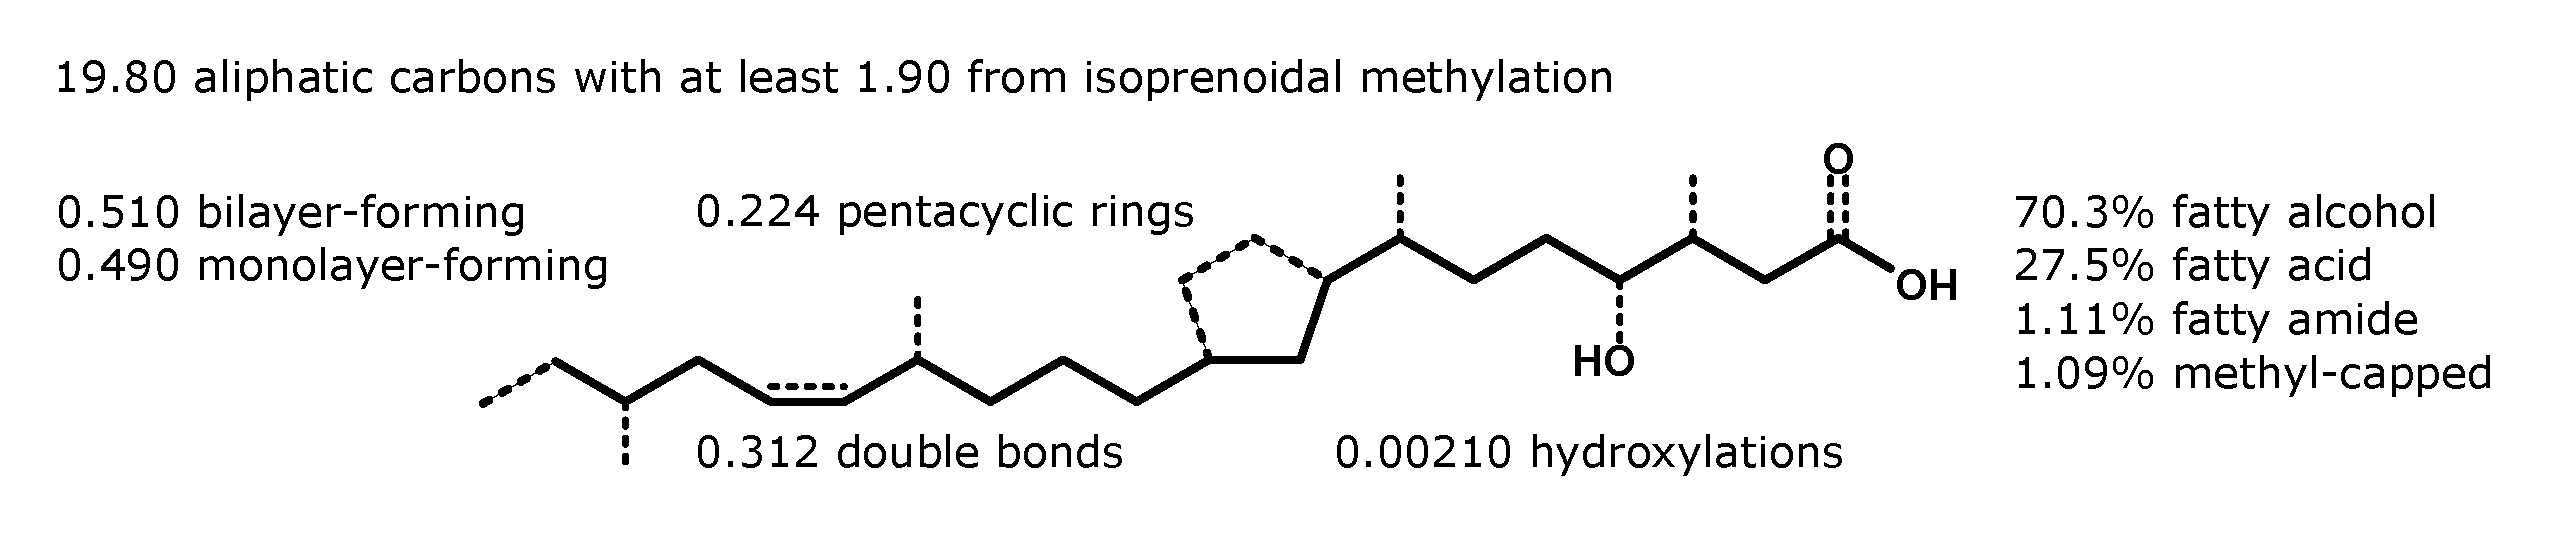
\includegraphics[width=\linewidth]{figs_ch2/sample_average_chain_Bison1}
\caption[Hypothetical chemical structure of the sample-averaged free alkyl chain of Bison Pool sample BP1]{Hypothetical chemical structure of the sample-averaged free alkyl chain of Bison Pool sample BP1 based on abundance-weighted structural characteristics of alkyl chains linked to observed intact polar lipids. Position and isomerism of hydroxylations, pentacyclic rings, methyl branches, and double bonds are not considered when calculating thermodynamic properties of sample-averaged free alkyl chains; their depiction here is to illustrate one of many possible interpretations of a hypothetical average molecule.}
\label{fig:ave_chain}
\end{figure}
\doublespace


\singlespace
\begin{figure}[h]
\centering

    \begin{subfigure}[b]{\linewidth}
      	\includegraphics[width=1\linewidth]{"figs_ch2/Bison OF1_thermo"}
      	\caption{BP1}
        \label{fig:BP1_thermo}
    \end{subfigure}
    \begin{subfigure}[b]{\linewidth}
    	\includegraphics[width=1\linewidth]{"figs_ch2/Bison OF2_thermo"}
    	\caption{BP2}
        \label{fig:BP2_thermo}
    \end{subfigure}
    
\end{figure}

\newpage

\begin{figure}[h]\ContinuedFloat
\centering

    \begin{subfigure}[b]{\linewidth}
      	\includegraphics[width=1\linewidth]{"figs_ch2/Bison OF3_thermo"}
      	\caption{BP3}
        \label{fig:BP3_thermo}
    \end{subfigure}
    \begin{subfigure}[b]{\linewidth}
    	\includegraphics[width=1\linewidth]{"figs_ch2/Bison OF4_thermo"}
    	\caption{BP4}
        \label{fig:BP4_thermo}
    \end{subfigure}
    
\end{figure}

\newpage

\begin{figure}[h]\ContinuedFloat

    \begin{subfigure}[b]{\linewidth}
    	\includegraphics[width=\linewidth]{"figs_ch2/Bison OF5_thermo"}
    	\caption{BP5}
        \label{fig:BP5_thermo}
    \end{subfigure}
    \begin{subfigure}[b]{\linewidth}
    	\includegraphics[width=\linewidth]{"figs_ch2/Bison OF6_thermo"}
    	\caption{BP6}
        \label{fig:BP6_thermo}
    \end{subfigure}
    
    \caption[Predicted metastable equilibrium abundance of sample-averaged free alkyl chains of Bison Pool samples]{Metastable equilibrium percent abundance of sample-averaged free alkyl chains of Bison Pool predicted across an Eh gradient at the temperatures and bicarbonate, ammonium, and proton concentrations measured at (a) BP1, (b) BP2, (c) BP3, (d) BP4, (e) BP5, and (f) BP6. Vertical dotted lines indicate lipid-predicted Eh for the sample.}
    \label{fig:bison_thermo}
\end{figure}
\doublespace


\singlespace
\begin{figure}[h]
\centering

    \begin{subfigure}[b]{\linewidth}
      	\includegraphics[width=1\linewidth]{"figs_ch2/boxplot_ggplot_02bin Bison OF1 iter 999"}
      	\caption{BP1}
        \label{fig:BP1_mc}
    \end{subfigure}
    \begin{subfigure}[b]{\linewidth}
    	\includegraphics[width=1\linewidth]{"figs_ch2/boxplot_ggplot_02bin Bison OF2 iter 999"}
    	\caption{BP2}
        \label{fig:BP2_mc}
    \end{subfigure}
    
\end{figure}

\newpage

\begin{figure}[h]\ContinuedFloat
\centering

    \begin{subfigure}[b]{\linewidth}
      	\includegraphics[width=1\linewidth]{"figs_ch2/boxplot_ggplot_02bin Bison OF3 iter 999"}
      	\caption{BP3}
        \label{fig:BP3_mc}
    \end{subfigure}
    \begin{subfigure}[b]{\linewidth}
    	\includegraphics[width=1\linewidth]{"figs_ch2/boxplot_ggplot_02bin Bison OF4 iter 999"}
    	\caption{BP4}
        \label{fig:BP4_mc}
    \end{subfigure}
    
\end{figure}
\doublespace



\singlespace
\begin{figure}[h]\ContinuedFloat

    \begin{subfigure}[b]{\linewidth}
    	\includegraphics[width=\linewidth]{"figs_ch2/boxplot_ggplot_02bin Bison OF5 iter 999"}
    	\caption{BP5}
        \label{fig:BP5_mc}
    \end{subfigure}
    \begin{subfigure}[b]{\linewidth}
    	\includegraphics[width=\linewidth]{"figs_ch2/boxplot_ggplot_02bin Bison OF6 iter 999"}
    	\caption{BP6}
        \label{fig:BP6_mc}
    \end{subfigure}
    
    \caption[Sensitivity analysis sample-averaged free alkyl chain metastable equilibrium percent abundance in Bison Pool samples]{Sensitivity analysis sample-averaged free alkyl chain metastable equilibrium percent abundance in Bison Pool samples (a) BP1, (b) BP2, (c) BP3, (d) BP4, (e) BP5, and (f) BP6 after 999 iterations of Monte Carlo-style random variation of lipid HPLC peak areas by 30\% and mass spectral response factors between 0.01x and 100x. Results have a resolution of 400 calculations per iteration, binned here into 0.02 volt increments. Dark horizontal lines indicate median values for each distribution, with 50\% of the results around the median falling within the colored box (interquartile range, or IQR). Whiskers extend to an observation 1.5 times the IQR beyond this range. Values that fall outside the span of the whiskers are not indicated to reduce visual clutter.}
    \label{fig:bison_mc}
\end{figure}
\doublespace


\singlespace
\begin{figure}[h]
\centering
\includegraphics[width=\linewidth]{"figs_ch2/scatterplot - alkyl chain predicted Eh"}
\caption[Alkyl chain-predicted Eh as a function of temperature and Eh]{Alkyl chain-predicted Eh as a function of temperature and Eh.}
\label{fig:alkyl_Eh}
\end{figure}
\doublespace